\documentclass[a4paper, doc]{apa6}
\usepackage[utf8]{inputenc}
\usepackage[ngerman]{babel}
\usepackage[T1]{fontenc}
\usepackage{setspace}
\onehalfspacing
\usepackage{amsmath}
\usepackage{amsfonts}
\usepackage{amssymb}
\usepackage{graphicx}
\usepackage{listings}
\usepackage{calc}
\usepackage{natbib}
\usepackage{lipsum}
\usepackage{todonotes}



\title{Projektbericht: Skin Cancer Detection}
\shorttitle{Skin Cancer Detection}
\author{Florence Lopez, Jonas Einig, Julian Späth }
\affiliation{Department of Computer Science, University of Tübingen}


\begin{document}

\maketitle
\begin{abstract}
In der Medizin unterscheidet man bei Hautverletzungen oder Hautveränderungen zwischen benignen und malignen Läsionen. Die malignen Läsionen gelten dabei als die bösartigen Hautveränderungen, die auf Hautkrebs hindeuten. Wir entwickelten daher auf der Grundlage einer anderen Arbeit einen Klassifikator, der aus einem Datensatz von Hautläsionen zwischen Benignen und Malignen unterscheidet. Durch diesen Klassifikator soll es zukünftig einfacher sein, bösartige Hautläsionen schneller zu erkennen, um diese effizient zu behandeln. Daher arbeiteten wir zusätzlich noch an einer mobilen Anwendung, welche es Nutzern ermöglicht, ihre Haut vorerst ohne eine ärztliche Analyse nach malignen und benignen Hautläsionen zu untersuchen. Natürlich kann eine solche Anwendung aber keinen Mediziner ersetzen, sondern lediglich als zusätzliche Unterstützung dienen. 
\end{abstract}
    
\section{Einleitung}

Hautkrebs gilt als eine der häufigsten Krebserkrankungen der Welt. Jährlich erkranken etwa 18.000 Menschen in Deutschland an dieser Krankheit, wobei Hautkrebs allgemein etwa für ein Prozent der Krebstodesfälle verantwortlich ist \citep{hautkrebs}. Findet eine Erkennung der malignen Hautläsionen frühzeitig statt, so ist es in den meisten Fällen möglich einen tödlichen Verlauf der Krankheit zu verhindern. Daher sind frühzeitige Erkennungssysteme sehr wichtig für die Bekämpfung von Hautkrebs.

Eine Ergänzung zum regelmäßigen Arztbesuch und dem damit verbundenem Hautscreening können daher neuronale Netze bieten, die aufgrund von medizinischen Datenbanken lernen zwischen malignen und benignen Hautläsion zu unterscheiden. Die genaue Implementierung und das Training eines solchen neuronalen Netzes werden wir in dieser Arbeit genauer erläutern. 
\section{Problemstellung und Zielsetzung}

Im Rahmen des Praktikums ``Maschinelles Lernen'' beschäftigen wir uns mit der folgenden Problemstellung: Ist es möglich einen Klassifikator zu entwickeln, der Bilder von Hautläsionen in maligne und benigne Läsionen unterteilen kann. Maligne Hautläsionen sind die Läsionen, die für den Menschen gefährlich bis sogar tödlich verlaufen können, während benigne Hautläsionen gutartig und ungefährlich sind. Unser Projekt basiert dabei auf der Arbeit von \citet{esteva2017dermatologist}, wobei wir die originale Problemstellung jedoch etwas abgewandelt haben. Während \citet{esteva2017dermatologist} viele verschiedene Arten von Hautläsionen unterschieden haben, unterscheiden wir lediglich binär, zwischen zwei Klassen, nämlich den gutartigen und den bösartigen Läsionen. Dies vereinfacht die Problemstellung.

Unser Ziel war es, eine möglichst hohe Genauigkeit zu erreichen und vor allem die Anzahl der falsch negativen Vorhersagen möglichst gering zu halten. Im Zweifel soll der Klassifikator eher eine Läsion als maligne klassifizieren, auch wenn sie eigentlich benigne ist, anstatt eine maligne Läsion, die tödlich verlaufen könnte, zu verharmlosen und als benigne zu klassifizieren. Im Folgenden werden wir genauer auf die Methodik eingehen, die hinter unserem Klassifikator steckt und welche Ergebnisse dieser auf unbekannten Bildern von Hautläsionen liefert. 
\section{Methoden und Tools}

Zur Erstellung des Klassifikators nutzten wir, wie \citet{esteva2017dermatologist} auch, das öffentlich zur Verfügung stehende GoogleNet Inception v3, welches ein \textit{convolutional neural network} ist und aus zahlreichen verschiedenen Schichten und Neuronen besteht \citep{szegedy2016rethinking}. Dieses neuronale Netz wurde auf den Bildern des \textit{ImageNet} vortrainiert \citep{russakovsky2015imagenet}. Die von uns genutzten Gewichte stammen aus der Tensorflow (\cite{tensorflow2015-whitepaper}) Bibliothek ``slim''.
Ein solches vorheriges Training auf ImageNet etabliert einige grundlegende Strukturen im neuronalen Netz. Es werden Merkmalsdetektoren gelernt, die anschließend in dem Training der eigentlichen Aufgabe verfeinert werden.  Das Training und die damit verbundene Vorverarbeitung implementierten wir mittels \textit{Python}, in Kombination mit \textit{Tensorflow} (\cite{tensorflow2015-whitepaper}), \textit{Scikit-Learn} (\cite{scikit-learn}) und \textit{NumPy}. Für die Evaluierung wurde außerdem noch Matlab verwendet.

Als Datensatz nutzten wir die ISIC-Datenbank (\cite{ISIC}), welche aus insgesamt 13.768 Bildern von sowohl malignen als auch benignen Hautläsionen besteht. Von den Datensätzen, die von \citet{esteva2017dermatologist} genutzt wurden, ist dieser der Einzige, welcher frei verfügbar ist. Die Bilder dieses Datensatzes sind durch eine pathologische Untersuchung gelabelt worden. Somit sind die vorhandenen Daten relativ zuverlässig. Wir teilten den Datensatz in drei Teildatensätze auf: einen Trainingsdatensatz, einen Validierungsdatensatz sowie einen Testdatensatz. Dabei beträgt der Anteil der Trainingsdaten $60\%$ und die Anteile der Validierungs- sowie der Testdaten jeweils $20\%$ aller Bilder. Diese wurden zufällig den Datensätzen zugeordnet.

Es stellte sich heraus, dass die Verteilung der Bilder dieses Datensatzes auf die verschiedenen Klassen (maligne/benigne) sehr unausgeglichen ist. Der Anteil der malignen Läsionen ist viel geringer als der Anteil der benignen Läsionen. Dieses Problem gingen wir durch eine spezielle Art der Randomisierung an. Während des Trainings trennten wir die Menge der Trainingsbilder in die Klassen \textit{maligne} und \textit{benigne} auf. Anschließend haben wir kleine Gruppen von Bildern, welche in das Netz gegeben wurden, aus Bildern dieser beiden Klassen zufällig befüllt. Dabei war die Wahrscheinlichkeit, dass ein Bild aus der Klasse der malignen Bilder stammt $p=0.5$. Somit wurde dieser unausgeglichene Datensatz ausbalanciert.

Ein weiteres Problem des ISIC-Datensatzes war die variable Größe der einzelnen Bilder. Für ein problemloses Trainieren des Netzes haben wir die Bilder daher vorverarbeitet. Dazu wurden die Bilder auf die kleinste verfügbare Größe skaliert. Für das Training des Netzes verwendeten wir, analog zu \citet{esteva2017dermatologist}, das maximale zentrale Quadrat des Bildes und skalierten es auf $299$px$\times 299$px herunter. Somit hatten wir eine homogene Menge an Bildern, die wir nun in einen Trainings-, Validierungs- und einen Testdatensatz unterteilten.

Während des Trainings wurden die Bilder zufällig augmentiert. Durch eine Augmentierung wird der Datensatz künstlich vergrößert, um mehr diverse Trainingsbeispiele für das neuronale Netz zu erhalten. Dazu wendet man eine klassenerhaltende Transformation auf das Bild an. In unserem Ansatz setzen wir viele verschiedene Augmentierungen ein, die jeweils zufällig auf ein Bild angewendet wurden. Abbildung~\ref{fig:aug} zeigt diese Augmentierungen anhand einer Beispielläsion.

\begin{figure}[t]
	\centering
	\begin{subfigure}[t]{0.24\linewidth}
		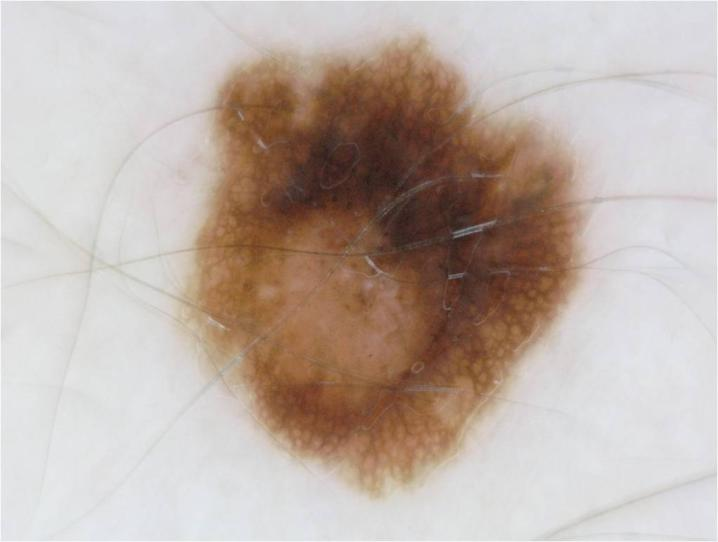
\includegraphics[width=\textwidth]{pics/augmentations/original.jpg}
		\caption{Original}
		\label{subfig:aug_original}
	\end{subfigure}
	\begin{subfigure}[t]{0.24\linewidth}
		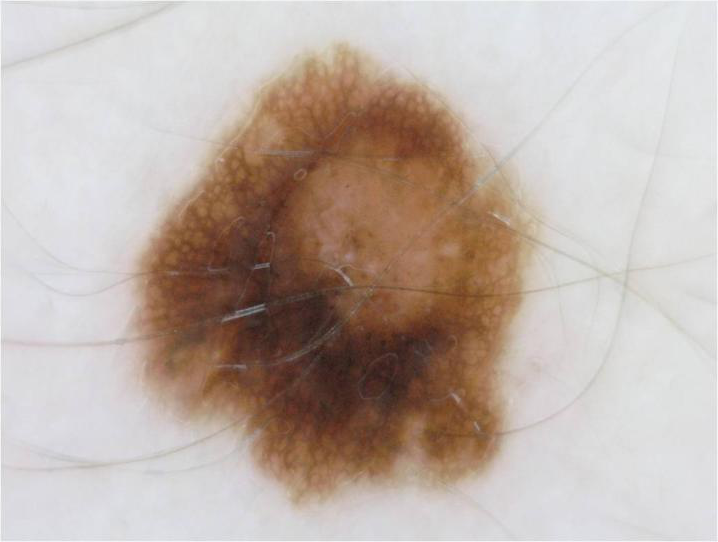
\includegraphics[width=\textwidth]{pics/augmentations/rotation.png}
		\caption{Rotation}
		\label{subfig:aug_rot}
	\end{subfigure}
	\begin{subfigure}[t]{0.24\linewidth}
		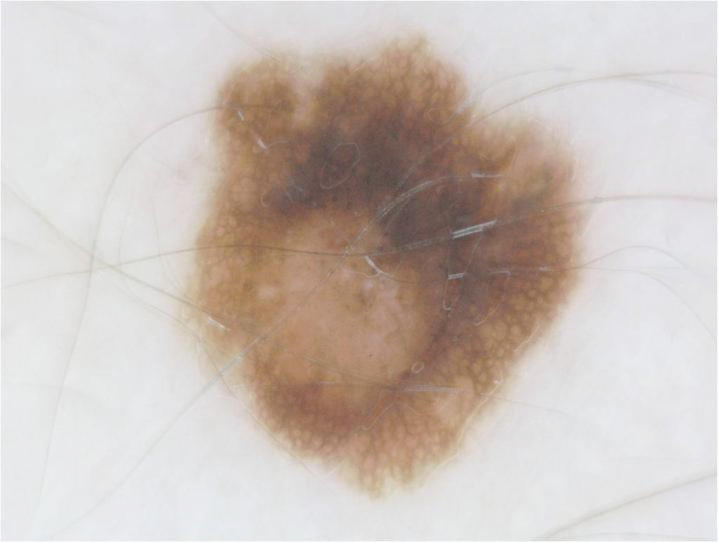
\includegraphics[width=\textwidth]{pics/augmentations/brightness.png}
		\caption{Helligkeit}
		\label{subfig:aug_bright}
	\end{subfigure}
	\begin{subfigure}[t]{0.24\linewidth}
		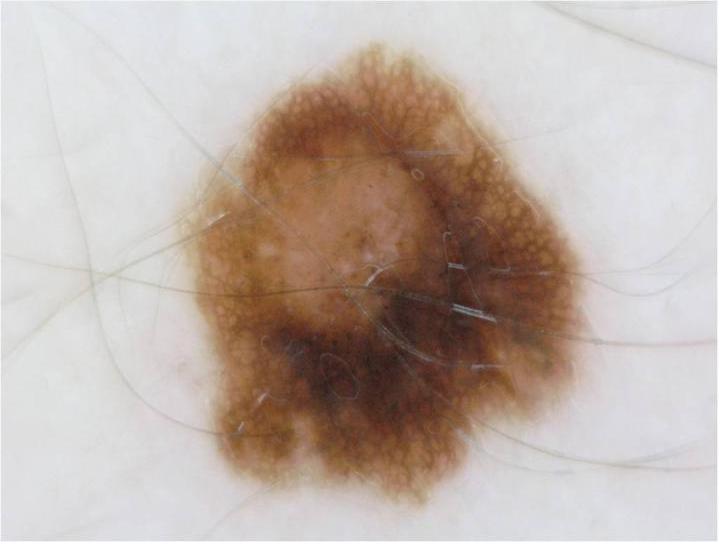
\includegraphics[width=\textwidth]{pics/augmentations/vertical_flip.png}
		\caption{Vertikale Spiegelung}
		\label{subfig:aug_v_flip}
	\end{subfigure}
	\begin{subfigure}[t]{0.24\linewidth}
		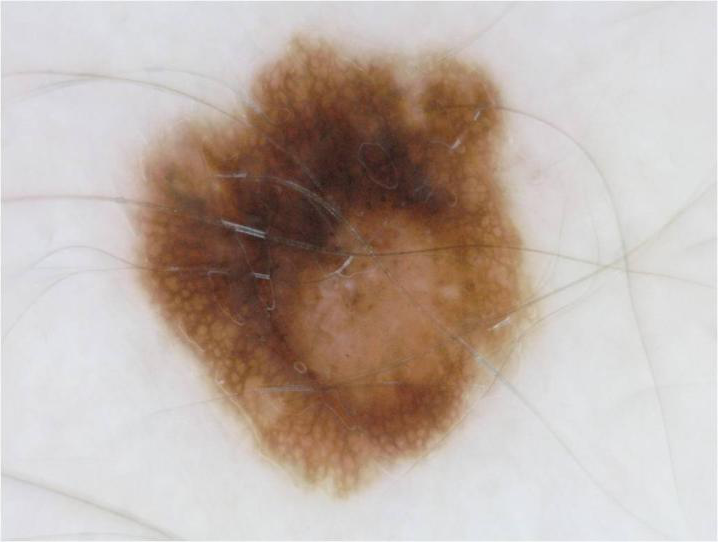
\includegraphics[width=\textwidth]{pics/augmentations/horizontal_flip.png}
		\caption{Horizontale Spiegelung}
		\label{subfig:aug_h_flip}
	\end{subfigure}
	\begin{subfigure}[t]{0.24\linewidth}
		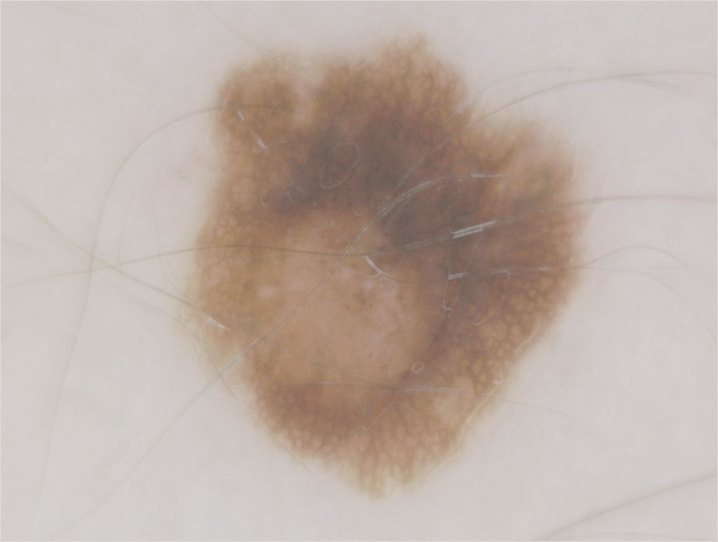
\includegraphics[width=\textwidth]{pics/augmentations/contrast.png}
		\caption{Kontrast}
		\label{subfig:aug_contrast}
	\end{subfigure}
	\begin{subfigure}[t]{0.24\linewidth}
		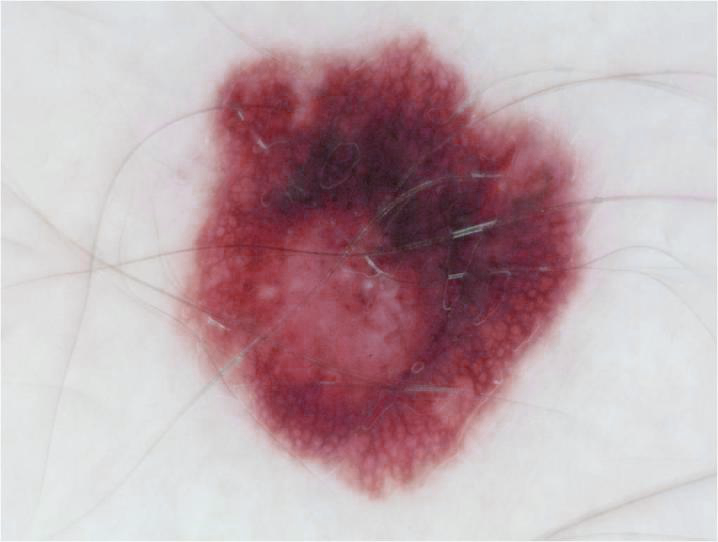
\includegraphics[width=\textwidth]{pics/augmentations/hue.png}
		\caption{Farbwert (Hue)}
		\label{subfig:aug_hue}
	\end{subfigure}
	\begin{subfigure}[t]{0.24\linewidth}
		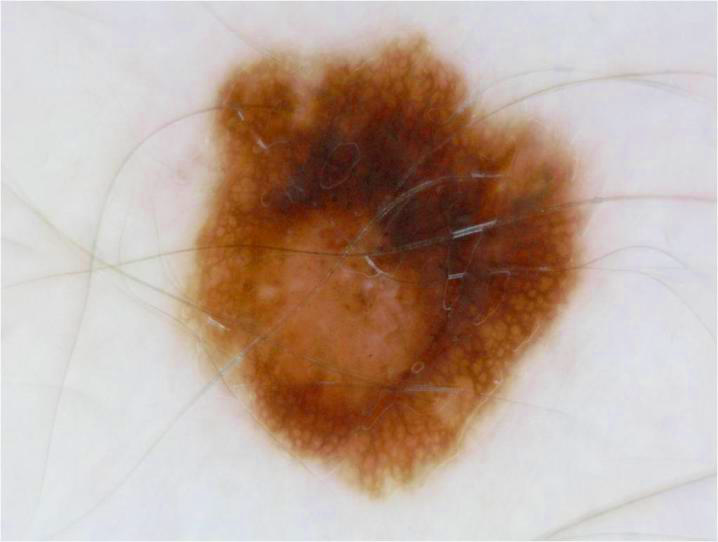
\includegraphics[width=\textwidth]{pics/augmentations/saturation.png}
		\caption{Sättigung}
		\label{subfig:aug_sat}
	\end{subfigure}
	\caption{Augmentierungsmethoden angewendet auf das originale Bild (\ref{subfig:aug_original})}
    \label{fig:aug}
\end{figure}


\begin{enumerate}
    \item \textbf{Rotation} (Abbildung \ref{subfig:aug_rot}): Bei dieser Transformation werden die Bilder je um 0$^{\circ}$, 90$^{\circ}$, 180$^{\circ}$ oder 270$^{\circ}$ gedreht. Diese Augmentierung soll das Netz invariant gegenüber Rotation machen. Dies ist wichtig, da die Orientierung der aufgenommenen Bilder willkürlich ist.
    
    \item \textbf{Helligkeit} (Abbildung \ref{subfig:aug_bright}):  Die Helligkeit der Bilder wird hier um einen zufälligen Wert erhöht oder verringert. So soll dem Netz eine gewisse Invarianz gegenüber verschiedenen Lichtbedingungen antrainiert werden.
    
    \item \textbf{Vertikales Spiegeln} (Abbildung \ref{subfig:aug_v_flip}): Bei dieser Methode werden die Bilder vertikal gespiegelt. Hierbei wird die Charakteristik der Läsion nicht verändert, jedoch werden so weitere Trainingsbilder erzeugt. 
    
    \item \textbf{Horizontales Spiegeln} (Abbildung \ref{subfig:aug_h_flip}):  In diesem Fall werden die Bilder horizontal gespiegelt. Auch hier wird die Charakteristik der Läsion nicht verändert, lediglich weitere Trainingsbilder erzeugt.
    
    \item \textbf{Kontrast} (Abbildung \ref{subfig:aug_contrast}):  Analog zur Helligkeit wird hier der Kontrast um einen zufälligen Wert erhöht oder erniedrigt. Auch dies soll das Netz invariant gegenüber wechselnden Lichtverhältnissen machen und zudem die Trainings-Menge vergrößern.
    
    \item \textbf{Farbwert (Hue)} (Abbildung \ref{subfig:aug_hue}):  Hier wird der Farbwert der Bilder zufällig verändert. Durch diese Methode soll die Unterscheidung der Klassen robuster gegenüber Farbänderungen in den Bildern gemacht werden.
    
    \item \textbf{Sättigung} (Abbildung \ref{subfig:aug_sat}):  Die Sättigung der Bilder wird zufällig um einen gewissen Wert verändert. Auch dies soll gegen abweichende Lichtverhältnisse helfen und die Menge der Trainingsdaten vergrößern.
\end{enumerate}

\subsection{Training}
\label{training}

	Das Training des GoogLeNet Inception v3 (\cite{inception}) implementierten wir in Tensorflow (\cite{tensorflow2015-whitepaper}). Dem Netz wurden Gruppen von jeweils sechs Bildern gezeigt. Von den augmentierten und zugeschnittenen Bildern wurde vor dem Inferenz-Schritt der Mittelwert der Bilder des ImageNet Datensatzes (\cite{russakovsky2015imagenet}) abgezogen. Dies ist ein gängiger Vorgang, um die Verteilung der RGB-Werte des ImageNet Datensatzes anzupassen. Nach einem Forward-Pass berechneten wir einen Loss. Auf diesem Loss trainierten wir das neuronale Netz mit dem \textit{Adam-Optimizer}. Im folgenden Abschnitt werden die getesteten Loss-Funktionen näher erläutert.
	
\subsubsection{L1-Loss}

	Dieser Loss berechnet die absolute Abweichung der Vorhersage von den wahren Labels:
	\begin{align*}
		L = \sum_{i = 0}^C \mid lab_i - x_i\mid
	\end{align*}
	Dabei ist $C$ die Anzahl der Klassen, $lab$ die wahren Labels und $x$ die Vorhersage des neuronalen Netzes.
	
	Das Ziel eines Trainings mit diesem Loss ist es, möglichst viele Nullen in dem Ergebnis-Vektor zu erhalten, da der L1-Loss spärliche (sparse) Lösungen begünstigt.

\subsubsection{L2-Loss}
	Dieser Loss berechnet die quadratische Abweichung der Vorhersage von den wahren Labels:
	\begin{align*}
	L = \sum_{i = 0}^C ( lab_i - x_i)^2
	\end{align*}
	Dabei ist $C$ die Anzahl der Klassen, $lab$ die wahren Labels und $x$ die Vorhersage des neuronalen Netzes.
	
	Das Ziel eines Trainings mit diesem Loss ist es, große Fehler stark zu bestrafen und die Abweichungen von den wahren Labels so klein wie möglich, jedoch nicht zwingend $=0$, zu halten.
	
\subsubsection{Softmax-Kreuzentropie-Loss}
	Dieser Loss nutzt das Maß der Kreuzentropie, um den Loss zu berechnen. Dabei wird zunächst die Softmax-Funktion auf die Vorhersage und die Labels angewendet und anschließend die Kreuzentropie der beiden Verteilungen berechnet.
	
	Dieser Loss wird dazu benutzt, um Verteilungen einander anzupassen. In unserem Ansatz verwendeten wir jedoch einen Vektor der Länge zwei als Klassenlabel. Bei solch einer kleinen Anzahl an Werten erwarteten wir, dass diese Loss-Funktion vergleichsweise schlecht abschneidet.
\\
\\
Um die oben angesprochene Unausgeglichenheit der Klassen in unserem Datensatz weiter zu balancieren und um eine bessere Performance für maligne Läsionen zu erreichen, nutzten wir bei dem L1-, wie auch bei dem L2-Loss zusätzlich einen Gewichtsterm. Dieser gewichtete die Abweichungen abhängig von der Zielklasse. Dabei wurden die Werte mit $lab=$ maligne mit $3$ und die Werte mit $lab=$ benigne mit $0.5$ multipliziert. 
	  

\subsection{Analysemethoden}
\label{analysemethoden}

Für die Bewertung und Optimierung unseres Klassifikators wurden verschiedene Methoden angewandt. Die Genauigkeit konnte mit unserem Datensatz nur unter großer Skepsis betrachtet werden. Sie berechnet sich durch die Anzahl der richtig vorhergesagten Stichproben dividiert durch die Anzahl aller Stichproben:
	\[\text{Accuracy} = \frac{TP+TN}{TP+TN+FP+FN}\]
Da der in diesem Projekt verwendete Datensatz deutlich mehr negative als positive Beispiele enthält, können unter dieser Berechnung sehr hohe Genauigkeiten auftreten, obwohl eventuell kein positives Beispiel richtig vorhergesagt wurde.
Eine weitaus bessere Analyse ist möglich, indem die richtig positiven und richtig negativen Beispiele getrennt betrachtet werden. Die Sensitivität, auch richtig-positiv-Rate oder auch Recall genannt, entspricht in unserem Fall dem Anteil an tatsächlich malignen Hautläsionen, bei denen diese auch als maligne erkannt wurden:
\[\text{Sensitivität} = \frac{TP}{TP+FN}\]
Die Spezifität, auch richtig-negativ-Rate genannt, entspricht dem Anteil an tatsächlich benignen Hautläsionen, die auch als benigne erkannt wurden:
\[\text{Spezifität} = \frac{TN}{TN+FP}\]
Die getrennte Betrachtung beider Werte erlaubt es uns direkt zu sehen, ob maligne oder benigne Beispiele besser erkannt werden und dementsprechend zu optimieren.

Zusätzlich zogen wir noch den \textit{Matthews correlation coefficient} in Betracht. Dieser wird als Qualitätsmaßstab in binären maschinellen Lernmethoden verwendet, im Speziellen wenn der Datensatz sehr unausgeglichen ist. 

\[\text{MCC} = \frac{TP*TN - FP*FN}{\sqrt{(TP+FP)*(TP+FN)*(TN+FP)*(TN+FN)}}\]

Im Gegensatz zu den anderen hier verwendeten Methoden, liefert der MCC Werte zwischen $-1$ und $1$. Ein MCC von $0$ ist somit nicht besser als eine Zufallsvorhersage. Ein MCC von $1$ hingegen steht für eine komplette Übereinstimmung, während $-1$ für die komplette Misklassifizierung steht.

Außerdem verwendeten wir noch den F2-Score als Qualitätsmaßstab. Der F1-Score ist das harmonische Mittel zwischen dem Recall und der Precision, der F2-Score dagegen gewichtet den Recall stärker und setzt somit den Schwerpunkt mehr auf die falsch negativen Stichproben, also die malignen Hautläsionen, die als benigne erkannt wurden:
	\[\text{Precision} = \frac{TP}{TP+FP}\]
    \[\text{Recall/Sensitivität} = \frac{TP}{TP+FN}\]
	\[\text{F1-Score} = 2*\frac{\text{precision}*\text{recall}}	{\text{precision}+\text{recall}}\]
   	\[\text{F2-Score} = 5*\frac{\text{precision}*\text{recall}}	{4*\text{precision}+\text{recall}}\]
    
Schließlich entschieden wir uns noch dazu, die \textit{Receiver-Operating-Characteristics-Kurve (ROC)} und die dazugehörige \textit{area under the curve (AUC)} zu verwenden. Diese Methode stellt visuell die Abhängigkeit der Sensitivität von der falsch-positiv-Rate dar. Eine ROC-Kurve nahe der Diagonalen deutet auf eine Zufallsvorhersage hin und hat eine AUC von $0.5$. Eine gute ROC-Kurve liegt deshalb oberhalb der Diagonalen und steigt senkrecht an bevor die falsch-positiv-Rate erhöht wird. Eine AUC von $1$ steht somit für eine perfekte Klassifizierung, eine AUC von $0$ für komplette Misklassifizierung. In diesem Falle könnten die Labels einfach umgedreht werden. Ziel ist es also eine ROC-Kurve weit entfernt von der Diagonalen zu erhalten.
    
Wir entschieden uns bewusst für eine größere Anzahl von Qualitätsmaßstäben. Da ein Parameter für sich nie die Komplexität des Klassifikators komplett beschreiben kann, sollen die verschiedenen Qualitätsmaßstäbe bei der Evaluierung und der Entscheidung für den für uns geeignetsten Klassifikator als Gesamtheit betrachtet und verwendet werden. Dies ermöglicht es uns, die Klassifizierung gezielt in die von uns gewünschte Richtung zu lenken, um beispielsweise falsch negative Vorhersagen zu minimieren.

\subsection{Framework}

Um sowohl das Training als auch die Evaluation auf verschiedenen Systemen durchführen und Parameteränderungen leicht über die Konsole testen zu können, entwickelten wir ein Framework. Über dieses Framework können Trainingsdurchläufe einfach gestartet und später automatisiert evaluiert werden. Dabei lassen sich die Trainingsparameter (Batchsize, Loss-Funktion, Lernrate, Datensatz), sowie plattformspezifische Einstellungen, wie der Speicherort der Daten und den Bezeichner der gewünschten Grafikkarte, anpassen. Startet man das Python-Skript ``start\_training.py'' mit den entsprechenden Parametern, wird automatisch ein neuronales Netz geladen und trainiert, sowie die Log-Dateien und die Gewichte entsprechend gespeichert. Für die Evaluation können analog die Systemparameter sowie der Datensatz, auf dem das Netzwerk evaluiert werden soll, eingestellt werden (Validierungsdatensatz oder Testdatensatz).



\section{Ergebnisse}

Um einen guten Klassfizierer zu bekommen, waren einige Trainingsdurchläufe notwendig. So kamen wir letzten Endes auf etwa 30 Trainingsdurchläufe, die jeweils einige Tage trainierten. Zur Parameteroptimierung für das Training wurden die trainierten Klassifizierer auf einen Validierungs-Datensatz angewandt, wobei die ersten Durchgänge dabei nur minimal bessere Ergebnisse als der Zufall geliefert haben. Durch verschiedene Anpassungen, die in Kapitel~\ref{training} näher erläutert wurden, konnten schließlich besser Ergebnisse erzielt werden. Einige ausgewählte Ergebnisse werden in Abbildung~\ref{fig:roc} als ROC-Kurve dargestellt. Jede Kurve steht für einen ausgewählten Klassifizierer und die entsprechende Anwendung auf den Validierungsdatensatz. Wie man gut erkennen kann, verlaufen zwei der Kurven nahe der Diagonalen. Die beiden Klassifikator (2018-03-12\_22-04-38 und 2018-03-12\_22-17-46) liefern somit keine guten Ergebnisse und sind nur etwas besser als eine zufällige Entscheidung. Gute Klassifikatoren verlaufen in der ROC-Kurve links oben und sind in diesem Fall 2018-03-10\_19-16-32, 2018-03-09\_21-34-4 und 2018-04-13\_20-38-20. Die anderen Klassifikatoren können auf den ersten Blick als in Ordnung eingestuft werden.

\begin{figure}[htb!]
	\begin{center}
		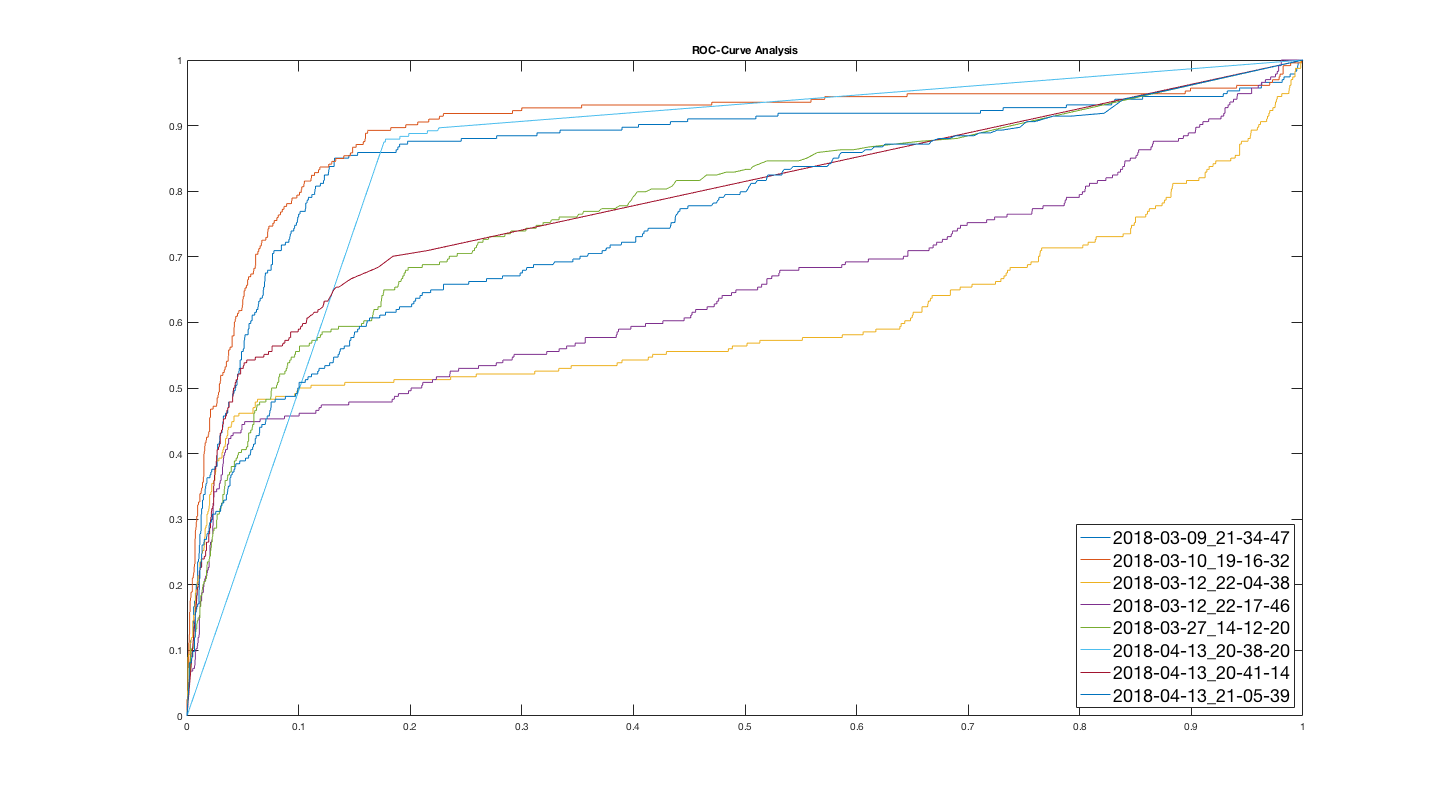
\includegraphics[width=\textwidth]{pics/roc_analysis.png}
		\caption{ROC-Kurven einiger trainierter Klassifizierer, angewandt auf den Validierungs-Datensatz.}
		\label{fig:roc}
    \end{center}
\end{figure}

Um die ROC-Kurve nicht nur optisch, sondern auf Grund von Fakten zu evaluieren, zeigt Tabelle~\ref{tab:auc} die Klassifikatoren aus Abbildung~\ref{fig:roc} zusammen mit ihrer berechneten AUC. Es ist deutlich zu erkennen, dass die Kurven, die links oben verlaufen, gleichzeitig eine höhere AUC aufweisen. Somit liefert der Klassifikator 2018-03-12\_22-04-38 mit einem AUC von $0.6$ die schlechteste Performance und ist nur leicht besser als eine Zufallsvorhersage. Der Klassifikator 2018-03-10\_19-16-32 hingegen hat mit einer AUC von $0.9$ die in diesem Fall beste Performance. 

\begin{table}[htb!]
\begin{center}
\begin{tabular}{ll}
	\toprule
 	Klassifikator  & AUC\\
	\midrule
  	2018-03-09\_21-34-47 &   $0.87$\\
    2018-03-10\_19-16-32 &   $0.90$\\
    2018-03-12\_22-04-38 &   $0.60$\\
    2018-03-12\_22-17-46 &   $0.65$\\
    2018-03-27\_14-12-20 &   $0.78$\\
    2018-04-13\_20-38-20 &   $0.86$\\
    2018-04-13\_20-41-14 &   $0.79$\\
    2018-04-13\_21-05-39 &   $0.75$\\
 \bottomrule
 \end{tabular}
 \end{center}
  \caption{ROC-AUC Ergebnisse einiger trainierten Klassifikatoren}
 \label{tab:auc}
 \end{table}
 
Da wir bei der Hautkrebs-Erkennung noch ein paar Sonderanforderungen an den Klassifikator haben und einen sehr unausgeglichenen Datensatz verwendeten, entschieden wir uns die zwei Klassifikatoren mit der höchsten AUC (2018-03-10\_19-16-32 und 2018-03-09\_21-34-47) noch genauer zu evaluieren. Unser Klassifizierer soll am Ende  eine hohe Vorhersagegenauigkeit haben, allerdings sollten nicht zu viele wirklich positive Ergebnisse (maligne) als negativ (benigne) klassifiziert werden. Unter Berücksichtigung wurden für dieses zwei Klassifikatoren noch weitere Qualitätsmaßstäbe berechnet. Tabelle~\ref{tab:scores} zeigt die verschiedenen Qualitätsmaßstäbe, die schon in Kapitel~\ref{analysemethoden} vorgestellt wurden. Wie man der Tabelle gut entnehmen kann, ist der Klassifikator 2018-03-10\_19-16-32 in nahezu allen Belangen besser als 2018-03-09\_21-34-47. Einzig und allein in der Spezifität weist er einen minimal schlechteren Wert auf.

\begin{table}[htb!]
\begin{center}
\begin{tabular}{lllllllllll}
	\toprule
 	Klassifikator  & TP & FN & TN & FP & MCC & F2 & Acc & Sens & Spez\\
	\midrule
	2018-03-09\_21-34-47 & $119$ &	$115$ &	$2406$ &	$113$ &	$0.47$ &	$0.51$&	$0.92$ &	$0.51$ & $0.96$\\
    2018-03-10\_19-16-32 & $142$&	$91$ &	$2406$ &	$114$ &	$0.54$ 	&$0.60$	&$0.93$	&$0.61$&	$0.95$ \\
 \bottomrule
 \end{tabular}
 \end{center}
  \caption{Scores der zwei besten Klassifizierer: TP = True Positives, FN = False Negatives, TN = True Negatives, FP = False Positives, MCC = Matthews Correlation Coefficient, F2 = F2-Score, Acc = Genauigkeit, Sens = Sensitivität und Spez = Spezifität }
 \label{tab:scores}
 \end{table}
 
Da unser Klassifikator maligne Hautläsionen auch wirklich als solche Erkennen soll präferieren wir in diesem Fall den, mit den wenigen falsch negativen und den mehr wirklich positiven Ergebnissen. Dabei wurde trotzdem nur ein negatives Ergebnis mehr fälschlicherweise als positiv (maligne) eingeordnet. Aufgrund dieser Evaluierung schlussfolgerten wir, dass der Klassifizierer mit der höheren AUC, Genauigkeit und Sensitivität sowie einem  höherem MCC und F2-Score unser Problem der Hautkrebserkennung besser lösen kann. Eine etwas geringere Spezifität nehmen wir hierbei in Kauf, wobei diese so gering ist, dass es sich auch um eine Zufallserscheinung handeln könnte.
 
Obwohl der Klassifizierer insgesamt schon gute Vorhersagen macht, werden die Ergebnisse durch die hohe Spezifität von $95\%$ etwas verfälscht. Mit einer Sensitivität von $0.6$ würden wir nämlich nur $60\%$ aller malignen Hautläsionen auch als wirklich maligne klassifizieren. Im Umkehrschluss heißt das, dass vier von zehn potentielle malignen Hautläsionen unerkannt bleiben. Da diese Sensitivität noch zu nah an einer Zufallsklassifizierung liegt, schauten wir uns die Ergebnisse des neuronalen Netzes des Klassifikators 2018-03-10\_19-16-32 noch einmal genauer an, da dieser in der vorherigen Evaluierung die besten Werte aufgewiesen hat. Das Ergebnis des neuronalen Netzes ist ein Score, der zwischen null und eins liegt. Ein Score über $0.5$ klassifiziert eine Hautläsion als maligne, ist er kleiner als $0.5$ als benigne. Um den Klassifizierer nun weiter in die von uns gewünschte Richtung zu lenken, verschoben wir die Entscheidungsschranke (Threshold) und schauten, wie sich diese Verschiebung auf die Klassifikation des Validierungsdatensatzes auswirkte. Diese Auswirkung auf die verschiedenen Qualitätsmaßstäbe wird in Abbildung~\ref{fig:threshold} dargestellt. 

\begin{figure}[htb!]
	\begin{center}
		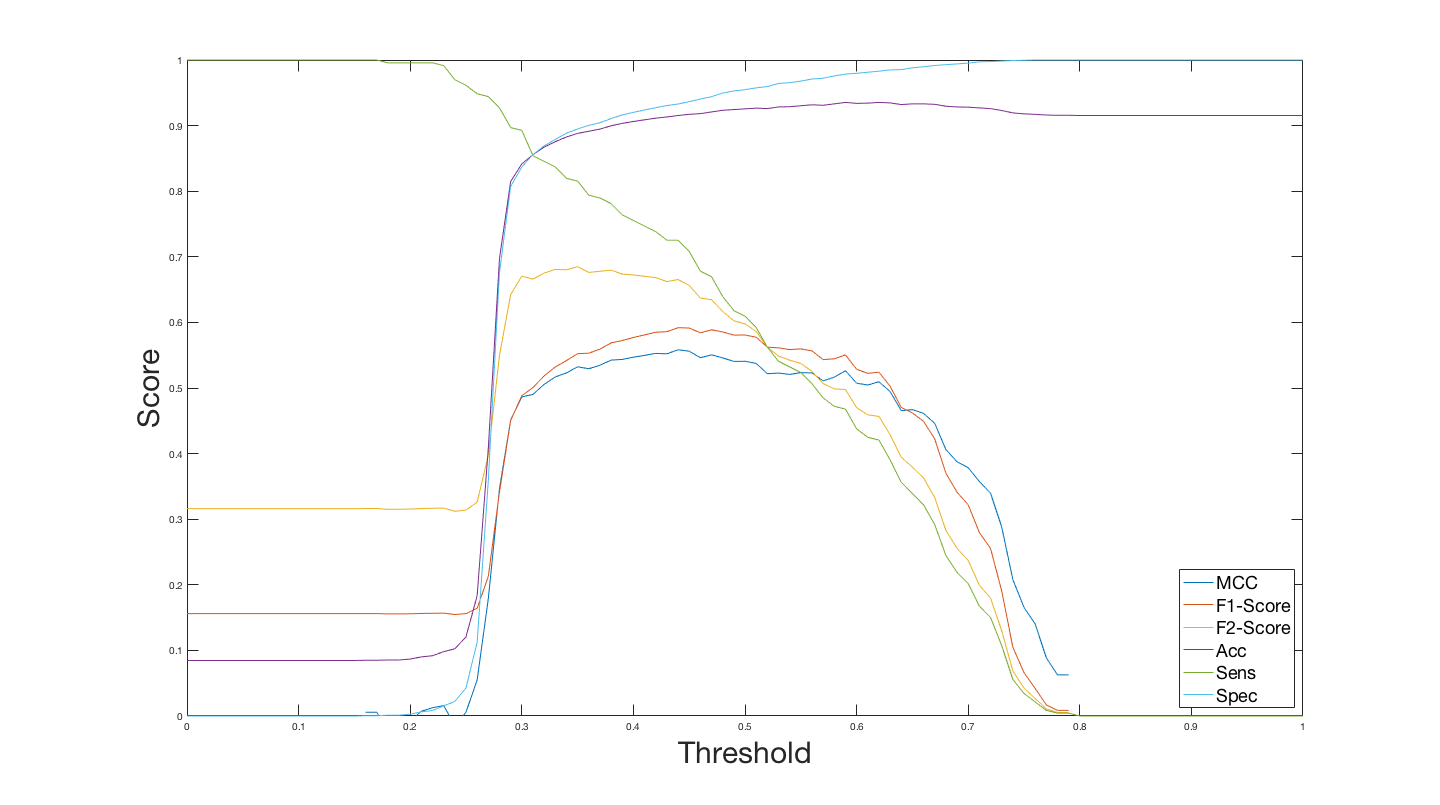
\includegraphics[width=\textwidth]{pics/treshold.png}
		\caption{Score-Threshold Abhängigkeit}
		\label{fig:threshold}
    \end{center}
\end{figure}

Wie man der Abbildung entnehmen kann, gibt es einen Bereich zwischen $0.3$ und $0.6$ in der der MCC und der F2-Score gute Werte aufweisen. Da der F2-Score die falsch negativen Stichproben noch stärker bestraft, konzentrierten wir uns hier mehr auf diesen Qualitätsmaßstab. Außerdem wollten wir eine möglichst hohe Sensitivität erreichen. Der F2-Score weist im Bereich $0.3$ und $0.45$ seine höchsten Werte auf, wobei der kleinste Threshold gleichzeitig die höchste Sensitivität liefert. Es wäre also naheliegend gewesen einfach diesen Wert zu nehmen. Da die Spezifität zwischen dem Threshold $0.25$ und $0.3$ rapide ansteigt, sollte allerdings ein gewisser Abstand zu diesem Bereich gewahrt werden. 

Abbildung~\ref{fig:verteilung} zeigt die Verteilung der Scores des Validierungsdatensatzes, der durch 2018-03-10\_19-16-32 klassifiziert wurde. Sie zeigt noch einmal deutlicher, dass die meisten benignen Stichproben einen Score zwischen $0.2$ und $0.3$ aufweisen. Somit entschieden wir uns den Threshold von den ursprünglichen $0.5$ auf $0.35$ herunterzusetzen. Damit halten wir genug Abstand von der extremen Änderung der Spezifität, klassifizieren gleichzeitig aber deutlich mehr maligne Stichproben richtig, ohne zu viele Fehler bei den negativen Stichproben zu machen. 

\begin{figure}[htb!]
	\begin{center}
		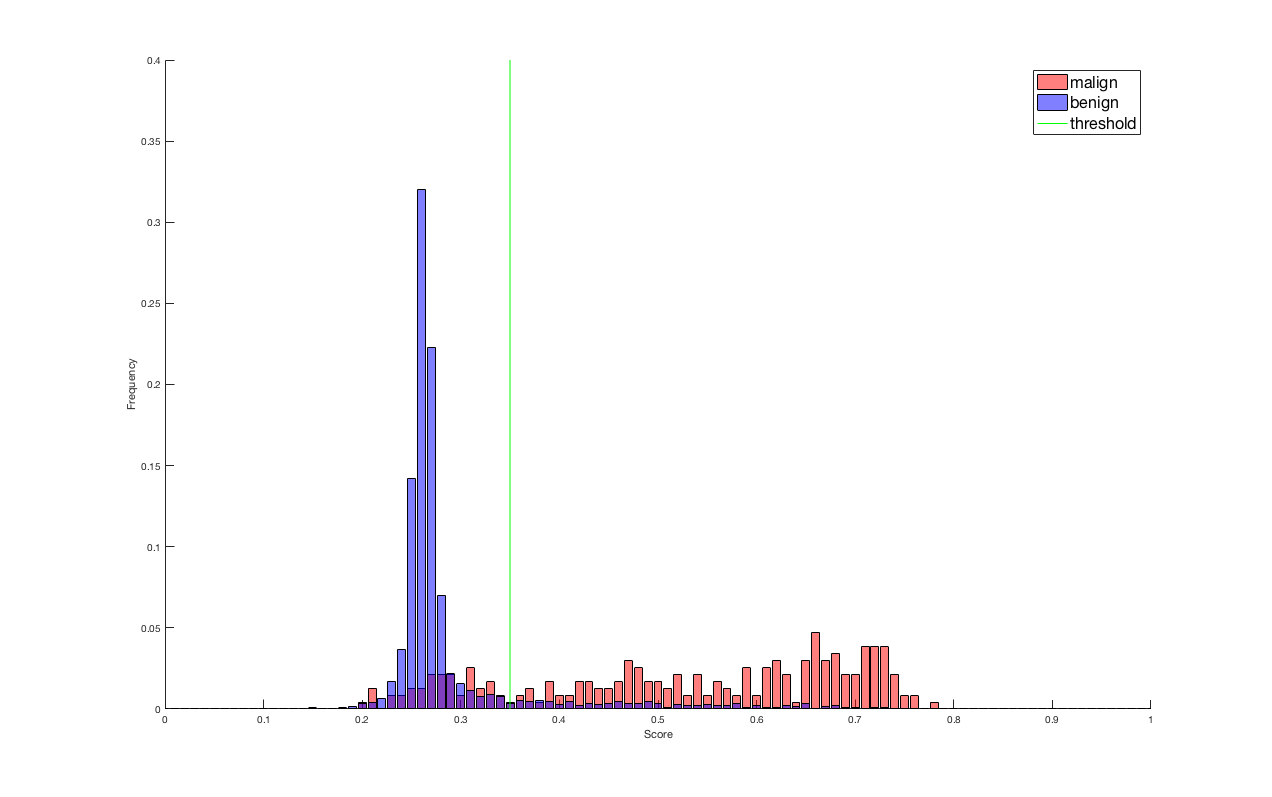
\includegraphics[width=\textwidth]{pics/score_threshold.png}
		\caption{Verteilung unserer Ergebnisse des Validierungs-Datensatzes. Maligne Beispiele werden in rot dargestellt, benigne in blau.}
		\label{fig:verteilung}
    \end{center}
\end{figure}


Durch diese nun sensitivere Klassifizierung erhielten wir schließlich die Werte, wie sie in Tabelle~\ref{tab:final_scores} gelistet sind. Die Sensitivität konnten wir durch die Verschiebung des Thresholds von $0.61$ auf $0.81$ erhöhen. Es werden also nur noch zwei von zehn maligne Hautläsionen fälschlicherweise benigne klassifiziert. Dabei akzeptierten wir eine Verringerung der Spezifität von $0.95$ auf $0.89$. Es wird also etwa jede zehnte benigne Hautläsion falsch als maligne klassifiziert. Die Genauigkeit verringerte sich dabei von $93\%$ auf $89\%$, allerdings erhöhten wir den F2-Score von $0.6$ auf $0.68$, der bei einem unausgeglichenen Datensatz höher zu gewichten ist als die Gesamtgenauigkeit.

\begin{table}[htb!]
\begin{center}
\begin{tabular}{lllllllllll}
	\toprule
 	Threshold  & TP & FN & TN & FP & MCC & F2 & Acc & Sens & Spez\\
	\midrule
    $0.5$ & $142$&	$91$ &	$2406$ &	$114$ &	$0.54$ 	&$0.60$	&$0.93$	&$0.61$&	$0.95$ \\
	$0.35$ & $190$ & $43$ &	$2255$ &	$265$ &	$0.55$ &	$0.68$&	$0.89$ &	$0.81$ & $0.89$\\
 \bottomrule
 \end{tabular}
 \end{center}
  \caption{Scores des Klassifikators mit dem Threshold bei $0.35$}
 \label{tab:final_scores}
 \end{table}

Unser bester Klassifikator 2018-03-10\_19-16-32 wurde mit einer Batchsize von sechs sowie einer Lernrate von $e^{-0.6}$ trainiert. Als Loss-Funktion verwendeten wir das L2-Loss. Als Entscheidungsschranke nahmen wir, wie oben beschrieben, $0.35$. Dies bedeutet, dass alle Stichproben, die einen Score von über $0.35$ erhalten, als maligne Hautläsionen eingestuft werden. Schließlich testeten wir unseren finalen Prädiktor noch auf unserem Testdatensatz. Dieser Datensatz wurde bis an diese Stelle isoliert aufbewahrt und keine der enthaltenen Daten waren dem Klassifikator bekannt. Dies war nötig, um zu testen, ob dieser auch generalisierbar ist. Das bedeutet, dass dieser nicht nur die Trainingsdaten auswendig gelernt hat, sondern auch auf nie gesehenen Daten gute Vorhersagen macht. Da wir anhand des Validierungsdatensatzes schon die Trainingsparameter angepasst haben, wurde dieser Testdatensatz jetzt am Schluss verwendet, um die endgültige Performance zu testen. Tabelle~\ref{tab:test_scores} zeigt die Qualitätsmaßstäbe, wie sie auf dem finalen Testdatensatz berechnet wurden.

\begin{table}[htb!]
\begin{center}
\begin{tabular}{lllllllllll}
	\toprule
 	TP & FN & TN & FP & MCC & F2 & Acc & Sens & Spez\\
	\midrule
    $149$&	$60$ &	$2285$ &	$114$ &	$0.48$ 	&$0.60$	&$0.88$	&$0.71$&	$0.9$ \\
 \bottomrule
 \end{tabular}
 \end{center}
  \caption{Qualität des Klassifikators nach Anwendung auf ungesehenen Trainingsdatensatz, mit der Entscheidungsgrenze bei $0.35$}
 \label{tab:test_scores}
 \end{table}

 Wie zu erwarten sind die Ergebnisse ähnlich, aber etwas schlechter als auf dem Validierungsdatensatz, auf dem wir gezielt auf gute Werte hingearbeitet haben. Letzten Endes erkennt unser Prädiktor $90\%$ der benignen Hautläsionen richtig und $71\%$ der malignen Hautläsionen. Der F2-Score ist mit $0.6$ auch etwas gesunken, was an den häufigeren falsch negativen Vorhersagen liegt.

Zusammenfassend kann man sagen, dass diese Werte auf jeden Fall in einem guten Bereich liegen. Die drei von zehn falsch negativen Vorhersagen sind zwar nicht erwünscht, aber auch durch den unausgeglichenen Datensatz zu begründen. Mit mehr malignen Trainingsdaten wären womöglich noch bessere Vorhersagen möglich. Nichtsdestotrotz erhielten wir nach unzähligen Trainings einen Prädiktor, der mit Vorsicht zur häuslichen Vorsorge verwendet werden kann und akzeptable Vorhersagen für die Hautkrebserkennung liefert.



\section{Aussicht und Diskussion}

Wie unsere Ergebnisse zeigen konnten, ist es durchaus möglich einen Klassifikator zu erstellen, der Bilder von Hautläsionen in maligne und benigne unterteilt. Dieser Klassifikator kann nun in verschiedenen Bereiche erfolgreich eingesetzt werden. Einen der Anwendungsbereiche betrachteten wir in unserem Projekt noch etwas genauer: Wir wollten den erstellten Klassifikator in eine mobile Anwendung einbinden, die es Nutzern ermöglicht, vorerst ohne ärztlichen Rat, ihre Haut auf Unregelmäßigkeiten und Anomalien zu untersuchen und eine vage Einschätzung dieser vorzunehmen. Dazu implementierten wir mittels Android Studio eine mobile Applikation, bei der ein Nutzer mittels seiner Handykamera ein Foto einer Hautläsion aufnehmen kann. Dieses kann anschließend durch unseren Klassifikator ausgewertet werden. 

Natürlich ist die Leistung, die eine solche mobile Anwendung bietet, ohne jegliche Gewähr, da eine Handykamera aufgrund ihrer geringeren Auflösung durchaus nicht einen ausgebildeten Hautarzt ersetzen kann. Trotzdem ist es durch diese Applikation möglich, eine erste Einschätzung des Hautzustandes vorzunehmen. Da wir weiterhin bei der Erstellung des Klassifikators sehr großen Wert darauf gelegt haben, vor allem die Rate der falsch negativen Vorhersagen zu minimieren, rät die mobile Anwendung dem Nutzer öfters dazu einen Hautarzt aufzusuchen, als es vielleicht wirklich nötig wäre. 

Zusätzlich könnte eine solche Mobile Applikation auch in Kombination mit einem speziellen Kamera-Aufsatz für präzise Aufnahmen der Haut genutzt werden. Damit wäre es möglich, die Genauigkeit der Klassifikation zu erhöhen und dadurch bessere Aussagen über den Gesundheitszustand des Nutzers zu treffen, da die Aufnahmen unseren Trainingsdaten noch mehr ähneln. Durch diese neue und einfache Art der Hautuntersuchung, wäre es vor allem auch Nutzern in ländlicheren Regionen, in denen ein Fachärzte-Mangel herrscht, möglich, eventuelle Unsicherheiten und Fragen bezüglich ihres Hautzustandes zu überprüfen. Obendrein birgt der Gebrauch von maschinellem Lernen in der Medizin in Kombination mit einer mobilen Anwendung einen weiteren großen Vorteil: Die Bevölkerung erhält dadurch die Gelegenheit sich von zu Hause aus mit wichtigen medizinischen Themen und Untersuchungen zu beschäftigen. Somit wird das Bewusstsein für schwere Krankheiten, wie zum Beispiel Hautkrebs, und die regelmäßige Auseinandersetzung mit ihnen gefördert. Infolgedessen wäre es möglich eine Prophylaxe vom eigenen Zuhause aus durchzuführen, was wiederum in einer frühzeitigen Erkennung von Anomalien und damit einhergehend, in einer schnellen und effizienten Behandlung dieser resultiert.

In unserem Projekt beschäftigten wir uns vorerst mit der allgemeinen Unterscheidung zwischen benignen und malignen Hautläsionen. Damit unterschied sich unsere Problemstellung von der des Originalpapers von \citet{esteva2017dermatologist} erheblich und wurde deutlich vereinfacht. Es wäre also in Zukunft möglich, die originale Fragestellung zu übernehmen und nicht nur zwischen benignen und malignen Hautläsionen, sondern auch zwischen den verschiedenen Unterklassen zu unterscheiden. Damit wäre es möglich, durch die mobile App eine genauere Einschätzung am Patienten vorzunehmen und die jeweils benötigte Medikation besser auf die klassifizierte Läsion einzustellen.

Abschließend konnten wir durch unser Projekt zeigen, dass es durch maschinelles Lernen möglich ist, bösartige Hautveränderungen frühzeitig als diese zu erkennen. Diese Art der Klassifizierung bringt in der Medizin viele Vorteile mit sich, nicht zuletzt, da es dem Patienten dadurch möglich wird, eine erste eigene Einschätzung des Gesundheitszustandes vorzunehmen. Natürlich kann die Richtigkeit einer solchen Klassifizierung nicht in dem Maße garantiert werden, in dem sie durch einen fachlich ausgebildeten Hautarzt gegeben ist, dennoch kann sie einen ersten Anhaltspunkt liefern und dazu führen, dass sich Patienten intensiver mit der Krankheit und ihrer Gesundheit auseinandersetzen. Vor allem durch die Einbindung des Klassifikators in eine benutzerfreundlichen mobile Applikation, kann der Vorteil des maschinellen Lernens in diesem Fall maximal ausgenutzt werden.  
 
\todo{App zustand --> fast fertig wird noch nachgeliefert auf github}
\color{red}

\begin{itemize}
	\item[\checkmark] Einbindung in App $\rightarrow$ unsere Fortschritte dort beschreiben
	\item[\checkmark] Verknüpfung des Klassifikators mit speziellen Kameras fürs Handy
	\item[\checkmark] Vorteil von ML in Medizin: Bewusstsein für Skin Cancer kann erhöht werden, einfachere Methode grad in ländlichen Gegenden (wo es nicht viele Ärzte gibt)
	\item[\checkmark] genauere Unterscheidung wie auch im Paper noch möglich (dass einzelne Subtypen auch erkannt und unterschieden werden)
	\item[\checkmark] Abschluss-Absatz

\end{itemize}
\color{black}

\bibliography{mylit}
\bibliographystyle{apalike}

\end{document}